%%
%% This is file `sample-xelatex.tex',
%% generated with the docstrip utility.
%%

%% The original source files were:
%%
%% samples.dtx  (with options: `sigconf')
%% 
%% IMPORTANT NOTICE:
%% 
%% For the copyright see the source file.
%% 
%% Any modified versions of this file must be renamed
%% with new filenames distinct from sample-sigconf.tex.
%% 
%% For distribution of the original source see the terms
%% for copying and modification in the file samples.dtx.
%% 
%% This generated file may be distributed as long as the
%% original source files, as listed above, are part of the
%% same distribution. (The sources need not necessarily be
%% in the same archive or directory.)
%%
%% The first command in your LaTeX source must be the \documentclass command.
\documentclass[sigconf]{acmart}
% Copyright 2017 Sergei Tikhomirov, MIT License
% https://github.com/s-tikhomirov/solidity-latex-highlighting/

\usepackage{listings, xcolor}

\definecolor{verylightgray}{rgb}{.97,.97,.97}

\lstdefinelanguage{Solidity}{
	keywords=[1]{anonymous, assembly, assert, balance, break, call, callcode, case, catch, class, constant, continue, constructor, contract, debugger, default, delegatecall, delete, do, else, emit, event, experimental, export, external, false, finally, for, function, gas, if, implements, import, in, indexed, instanceof, interface, internal, is, length, library, log0, log1, log2, log3, log4, memory, modifier, new, payable, pragma, private, protected, public, pure, push, require, return, returns, revert, selfdestruct, send, solidity, storage, struct, suicide, super, switch, then, this, throw, transfer, true, try, typeof, using, value, view, while, with, addmod, ecrecover, keccak256, mulmod, ripemd160, sha256, sha3}, % generic keywords including crypto operations
	keywordstyle=[1]\color{blue}\bfseries,
	keywords=[2]{address, bool, byte, bytes, bytes1, bytes2, bytes3, bytes4, bytes5, bytes6, bytes7, bytes8, bytes9, bytes10, bytes11, bytes12, bytes13, bytes14, bytes15, bytes16, bytes17, bytes18, bytes19, bytes20, bytes21, bytes22, bytes23, bytes24, bytes25, bytes26, bytes27, bytes28, bytes29, bytes30, bytes31, bytes32, enum, int, int8, int16, int24, int32, int40, int48, int56, int64, int72, int80, int88, int96, int104, int112, int120, int128, int136, int144, int152, int160, int168, int176, int184, int192, int200, int208, int216, int224, int232, int240, int248, int256, mapping, string, uint, uint8, uint16, uint24, uint32, uint40, uint48, uint56, uint64, uint72, uint80, uint88, uint96, uint104, uint112, uint120, uint128, uint136, uint144, uint152, uint160, uint168, uint176, uint184, uint192, uint200, uint208, uint216, uint224, uint232, uint240, uint248, uint256, var, void, ether, finney, szabo, wei, days, hours, minutes, seconds, weeks, years},	% types; money and time units
	keywordstyle=[2]\color{teal}\bfseries,
	keywords=[3]{block, blockhash, coinbase, difficulty, gaslimit, number, timestamp, msg, data, gas, sender, sig, value, now, tx, gasprice, origin},	% environment variables
	keywordstyle=[3]\color{violet}\bfseries,
	identifierstyle=\color{black},
	sensitive=false,
	comment=[l]{//},
	morecomment=[s]{/*}{*/},
	commentstyle=\color{gray}\ttfamily,
	stringstyle=\color{red}\ttfamily,
	morestring=[b]',
	morestring=[b]"
}

\lstset{
	language=Solidity,
	backgroundcolor=\color{verylightgray},
	extendedchars=true,
	basicstyle=\footnotesize\ttfamily,
	showstringspaces=false,
	showspaces=false,
	numbers=left,
	numberstyle=\footnotesize,
	numbersep=9pt,
	tabsize=2,
	breaklines=true,
	showtabs=false,
	captionpos=b
}
\usepackage{bera}% optional: just to have a nice mono-spaced font

\colorlet{punct}{red!60!black}
\definecolor{background}{HTML}{EEEEEE}
\definecolor{delim}{RGB}{20,105,176}
\colorlet{numb}{magenta!60!black}

\lstdefinelanguage{json}{
    basicstyle=\normalfont\ttfamily,
    numbers=left,
    numberstyle=\scriptsize,
    stepnumber=1,
    numbersep=8pt,
    showstringspaces=false,
    breaklines=true,
    frame=lines,
    backgroundcolor=\color{background},
    literate=
     *{0}{{{\color{numb}0}}}{1}
      {1}{{{\color{numb}1}}}{1}
      {2}{{{\color{numb}2}}}{1}
      {3}{{{\color{numb}3}}}{1}
      {4}{{{\color{numb}4}}}{1}
      {5}{{{\color{numb}5}}}{1}
      {6}{{{\color{numb}6}}}{1}
      {7}{{{\color{numb}7}}}{1}
      {8}{{{\color{numb}8}}}{1}
      {9}{{{\color{numb}9}}}{1}
      {:}{{{\color{punct}{:}}}}{1}
      {,}{{{\color{punct}{,}}}}{1}
      {\{}{{{\color{delim}{\{}}}}{1}
      {\}}{{{\color{delim}{\}}}}}{1}
      {[}{{{\color{delim}{[}}}}{1}
      {]}{{{\color{delim}{]}}}}{1},
}
\usepackage{listings}
\usepackage{xcolor}

\definecolor{codegreen}{rgb}{0,0.6,0}
\definecolor{codegray}{rgb}{0.5,0.5,0.5}
\definecolor{codepurple}{rgb}{0.58,0,0.82}
\definecolor{backcolour}{rgb}{0.95,0.95,0.92}

\lstdefinestyle{mystyle}{
    backgroundcolor=\color{backcolour},   
    commentstyle=\color{codegreen},
    keywordstyle=\color{magenta},
    numberstyle=\tiny\color{codegray},
    stringstyle=\color{codepurple},
    basicstyle=\ttfamily\footnotesize,
    breakatwhitespace=false,         
    breaklines=true,                 
    captionpos=b,                    
    keepspaces=true,                 
    numbers=left,                    
    numbersep=5pt,                  
    showspaces=false,                
    showstringspaces=false,
    showtabs=false,                  
    tabsize=2
}

\lstset{style=mystyle}
%% NOTE that a single column version may be required for 
%% submission and peer review. This can be done by changing
%% the \doucmentclass[...]{acmart} in this template to 
%% \documentclass[manuscript,screen]{acmart}
%% 
%% To ensure 100% compatibility, please check the white list of
%% approved LaTeX packages to be used with the Master Article Template at
%% https://www.acm.org/publications/taps/whitelist-of-latex-packages 
%% before creating your document. The white list page provides 
%% information on how to submit additional LaTeX packages for 
%% review and adoption.
%% Fonts used in the template cannot be substituted; margin 
%% adjustments are not allowed.
%%
%%
%% \BibTeX command to typeset BibTeX logo in the docs
\AtBeginDocument{%
  \providecommand\BibTeX{{%
    \normalfont B\kern-0.5em{\scshape i\kern-0.25em b}\kern-0.8em\TeX}}}

%% Rights management information.  This information is sent to you
%% when you complete the rights form.  These commands have SAMPLE
%% values in them; it is your responsibility as an author to replace
%% the commands and values with those provided to you when you
%% complete the rights form.
\setcopyright{acmcopyright}
\copyrightyear{2018}
\acmYear{2018}
\acmDOI{XXXXXXX.XXXXXXX}

%% These commands are for a PROCEEDINGS abstract or paper.
\acmConference[Conference acronym 'XX]{Make sure to enter the correct
  conference title from your rights confirmation emai}{June 03--05,
  2018}{Woodstock, NY}
%
%  Uncomment \acmBooktitle if th title of the proceedings is different
%  from ``Proceedings of ...''!
%
%\acmBooktitle{Woodstock '18: ACM Symposium on Neural Gaze Detection,
%  June 03--05, 2018, Woodstock, NY} 
\acmPrice{15.00}
\acmISBN{978-1-4503-XXXX-X/18/06}


%%
%% Submission ID.
%% Use this when submitting an article to a sponsored event. You'll
%% receive a unique submission ID from the organizers
%% of the event, and this ID should be used as the parameter to this command.
%%\acmSubmissionID{123-A56-BU3}

%%
%% The majority of ACM publications use numbered citations and
%% references.  The command \citestyle{authoryear} switches to the
%% "author year" style.
%%
%% If you are preparing content for an event
%% sponsored by ACM SIGGRAPH, you must use the "author year" style of
%% citations and references.
%% Uncommenting
%% the next command will enable that style.
%%\citestyle{acmauthoryear}

%%
%% end of the preamble, start of the body of the document source.
\begin{document}

%%
%% The "title" command has an optional parameter,
%% allowing the author to define a "short title" to be used in page headers.
\title{Solidity Smart Contracts: Language constructs for control/currency exchange and guards}

%%
%% The "author" command and its associated commands are used to define
%% the authors and their affiliations.
%% Of note is the shared affiliation of the first two authors, and the
%% "authornote" and "authornotemark" commands
%% used to denote shared contribution to the research.
\author{Darin Verheijke}
\email{darin.verheijke@student.uantwerpen.be}
\affiliation{%
  \institution{University of Antwerp}
  \city{Antwerp}
  \country{Belgium}
}



%%
%% By default, the full list of authors will be used in the page
%% headers. Often, this list is too long, and will overlap
%% other information printed in the page headers. This command allows
%% the author to define a more concise list
%% of authors' names for this purpose.
\renewcommand{\shortauthors}{Trovato and Tobin, et al.}

%%
%% The abstract is a short summary of the work to be presented in the
%% article.
\begin{abstract}
    Ethereum is a blockchain platform which enables the use of smart contracts. Smart contracts will execute a set of instructions without intermediary party when called upon, this process happens automatically. The possibility to make calls to another smart contract within a contract allows for potential exploits to occur. In this paper we will discuss and look at how one of these exploits, called the reentrancy attack, is possible. This attack is most well known for The DAO attack in 2016 where almost 55 million dollar got drained by an attacker who made use of this vulnerability in the smart contract. More specifically we will look at the concept in the Solidity programming language which was made specifically for the Ethereum blockchain. Also an overview of the different advantages and disadvantages of the different functions to exchange Ether, the currency used to execute transactions, will be given, how they work and how the call function might allow for certain exploits. The reentrancy vulnerability is still prevalent in smart contracts nowadays and forms a huge threat to applications and their users due to the huge possible financial losses that can happen. This research also includes an analysis of a verified smart contract database that was collected from Etherscan. This was done to detect potential vulnerabilities by looking for the presence of functions that allow for these attacks. Finally, the results of this analysis are discussed and there will be a brief discussion about prevention measures and methods to avoid a reentrancy attack.
\end{abstract}

%%
%% The code below is generated by the tool at http://dl.acm.org/ccs.cfm.
%% Please copy and paste the code instead of the example below.
%%
\begin{CCSXML}
<ccs2012>
   <concept>
       <concept_id>10002978</concept_id>
       <concept_desc>Security and privacy</concept_desc>
       <concept_significance>500</concept_significance>
       </concept>
   <concept>
       <concept_id>10002978.10002979</concept_id>
       <concept_desc>Security and privacy~Cryptography</concept_desc>
       <concept_significance>500</concept_significance>
       </concept>
   <concept>
       <concept_id>10002978.10003006.10003013</concept_id>
       <concept_desc>Security and privacy~Distributed systems security</concept_desc>
       <concept_significance>500</concept_significance>
       </concept>
   <concept>
       <concept_id>10002978.10003022.10003023</concept_id>
       <concept_desc>Security and privacy~Software security engineering</concept_desc>
       <concept_significance>500</concept_significance>
       </concept>
 </ccs2012>
\end{CCSXML}

\ccsdesc[500]{Security and privacy}
\ccsdesc[500]{Security and privacy~Cryptography}
\ccsdesc[500]{Security and privacy~Distributed systems security}
\ccsdesc[500]{Security and privacy~Software security engineering}
%%
%% Keywords. The author(s) should pick words that accurately describe
%% the work being presented. Separate the keywords with commas.
\keywords{blockchain, smart contracts, solidity, ethereum, reentrancy}


%%
%% This command processes the author and affiliation and title
%% information and builds the first part of the formatted document.
\maketitle

\section{Introduction}
A blockchain is an append-only transactional database where the information is structured together in groups, also known as blocks \cite{smart_inspect}\cite{smarter}. Each block has certain storage capacities and is chained onto the previous filled block, thus forming a blockchain. Another way to define it is a shared, immutable ledger that records transactions which can be used to track different assets. Most notable uses of this blockchain technology are the cryptocurrencies Bitcoin\cite{article} and Ether \cite{ethereum}\cite{white_paper} on the Ethereum network. One important difference between these two blockchain platforms is that Ethereum enables the deployment of smart contracts. 

A smart contract is a contract which executes automatically when called upon where the terms between the two parties is written in code (on the blockchain). These contracts then run when a function is called and the conditions for that function are met and can be used to automate executions of agreements without any intermediary party \cite{criminal}\cite{10.1145/2993600.2993611}\cite{smarter}. In their simplest form a contract is just a collection of functions. Interesting to note is that all smart contract transactions are traceable, transparent and also irreversible \cite{smart_inspect}\cite{smarter}.

A common functionality of smart contracts is the possibility to make calls to another contract on the same blockchain platform. This however needs to be done with caution as untrusted contracts can not only introduce errors but also risks as the contract or call may execute malicious code and exploit vulnerabilities. Every call transfers execution control to the called contract.

One of these dangers when calling an external contract is called Reentrancy and is one of the most well known attacks due to the DAO Attack on June 17th 2016 where around 3.6 million Ether was taken which equated to around \$50 million dollar at the time \cite{10.1007/978-3-662-54455-6_8}. This exploit is cemented in the history of Ethereum as it resulted into Ethereum being forked into Ethereum Classic and the Ethereum we know today. The original version of this attack involved functions that would be called repeatedly before the first function was finished. 

Solidity is one of the major programming languages for smart contracts on Ethereum. To avoid these exploits there have been introduced some best practices. More specifically the function call() was to be replaced by the more safe functions transfer() and send(). However, recently there has been a switch back to the call() function with the introduction of EIP 1884 \cite{eip1884}. Other precautions instead must be taken to prevent reentrancy attacks, one recommendation is making use of a checks-effects-interactions pattern. 

In this research internship we will investigate how these calling functions are used in practice and if they are still commonly used in the current smart contracts. For this we have collected a database of 28414 unique open-source verified smart contracts from Etherscan (dating from July 7th 2021 up until January 6th 2022) to perform our research.

In this research, we expect to find patterns on how contracts use call functions and to potentially find contracts that still include functions that are to be avoided for exploits.
\section{Background}
An introduction to some important concepts such as blockchain, the consensus mechanism used in Ethereum, smart contracts and reentrancy attacks is given. The scope of these concepts will be kept to the Ethereum blockchain and one of its programming languages Solidity \cite{solidity}.
\subsection{Blockchain}
A blockchain is a decentralized, distributed and immutable ledger that differs from a typical database in the way that it stores information. All recorded transactions, structured in blocks, are linked together using cryptography. Each block will contain a hash of the previous block, a timestamp and transaction data. As each block contains information from the previous block due to the hash, they will form a chain, thus forming a blockchain \cite{article}. It is a peer-to-peer network connecting participants. These participants will be forced to cooperate using a consensus mechanism which enforces rules in order to decentralize control.
\subsection{Consensus mechanisms}
A blockchain reaches consensus when at least 51\% of the nodes on the network agree on the next state of the network. These consensus mechanisms are designed to prevent 51\% attacks on the network. Executing a 51\% attack would require the attacker to have 51\% of the nodes on the network which is considered theoretically impossible due to the decentralized nature of a blockchain but would allow the attacker to decide on the next state of the network by himself due to controlling over half of the nodes and thus choosing which state is correct. Currently, Ethereum uses a proof-of-work consensus mechanism which defines the work that miners (network operators) have to do add a new valid block to the chain. The 'work' they do is a cryptographic math puzzle where the winner (i.e. the fastest to solve the puzzle) earns a reward and shares the new block with the rest of the network. This concept is called 'mining' and has as purpose to secure the blockchain with as incentive newly minted currency of the respective blockchain as a way to reward those who contribute to the system. There has been some criticism on POW due to the amount of energy used and needed to keep the network safe. The Ethereum network consumes 73.2 TWh annually which is comparable to the amount of energy used in Belgium which is 82.16 TWh. Ethereum thus plans to move to proof-of-stake which at a high level has the same end-goal as POW. Very briefly explained, miners will be replaced with validators who can stake their Ether to activate the ability to create new blocks. This consensus mechanism should also have a stronger immunity to centralization as POS should lead to more nodes in the network. For more information on the POS consensus mechanism and Ethereum their change to it we refer to the documentation \cite{ethereum}  \cite{white_paper}.
\subsection{Ethereum \& Smart contracts}
Ethereum differs from Bitcoin in that it enables the deployment of smart contracts and decentralized applications also known as dApps with built-in economic functions. While bitcoin its primary focus is to be a digital currency payment network, Ethereum is designed to be a general-purpose programmable blockchain that runs a virtual machine capable of executing code.
Ether is the currency used to complete transactions on the network and is used as a way to meter and constrain execution resource costs. In comparison to bitcoin, Ether is designed to be a utility currency which is used to call transactions on the Ethereum platform as a sort of fee \cite{mastering}.  Ethereum has two account types, Externally-owned accounts and contracts. Externally-owned accounts can be controlled by anyone who has the private keys to this account while smart contracts are deployed to the network and are controlled by code. Smart contracts can be used to create a range of dApps. In this paper we will focus on the smart contract itself which in its most basic form is a piece of code that runs on the blockchain and guarantees the same output for everyone that runs them. An important feature of smart contracts is that when a function is called and the conditions for that function are met there is an automatic execution of the set agreements without any intermediary party \cite{ethereum} \cite{white_paper}.

We take a look at the vending machine example introduced by Nick Szabo, who first coined the term 'Smart contract'\cite{nick}. A simple vending machine will take in coins and via a simple mechanism dispense change and the output we selected. How a vending machine removes the need for a vendor employee, smart contracts remove the intermediary party. Some important properties of smart contracts is that they are immutable and deterministic. Immutable because once deployed due to the nature of how a blockchain works, the code can not change of the smart contract. The only way to modify a smart contract is to deploy a new instance (and thus a new smart contract). Deterministic in the way the outcome after is identical for everyone who, given the same transaction parameters and state of the Ethereum blockchain, executes the contract \cite{white_paper}.

Important to note, contracts are only run if they are called by a transaction. A contract can call another contract that in its turn can then call another contract however the first part of this chain will always be a transaction called by an Externally-owned account. All transactions will either successfully terminate or revert. While a contract can not be changed, it can be deleted, removing the code and its storage from its address leaving an empty account. Any transactions sent there will not result in any execution of code. 

Executing a transaction requires a fee which is called the gas fee. It refers to the amount of computational effort required to execute specific operations, these fees are paid in Ether. It's part of the reward miners get in exchange for their service. Gas prices are denoted in gwei which is equal to $10^{-9}$ Ether. These fees help keep the network secure by preventing bad actors from spamming the network \cite{docs}.

Anybody with enough Ether can deploy and write a smart contract to the network. Deployment of a smart contract is also considered a transaction and thus also requires a gas fee.
\subsection{Solidity}
One of those smart contract languages in which contracts are coded is Solidity, which is an object-oriented, high-level language which has syntax comparable to C++. We won't go in the details of this programming language but instead will look at and describe the call, send and transfer functions which will be relevant for understanding the research and analysis made later in this paper, all of these three functions are used as a way to exchange Ether.

The call function is a low-level interface for sending a message to a contract and is a way to send Ether via calling the fallback function, the call function allows for some vulnerabilities which we will go more in depth about later. The send function also made it possible to send an amount to a specific address however it has two small issues. Only a small amount of gas is sent along, which allows for only one single event at max and thus it can't be a contract that changes state variables or does another call to another contract. While this does make it safe, it does cause developers to default back to the unsafe call function to implement calls to other contracts. The other issue it had is that an error would return false instead of propagating the error. The transfer function was introduced which fully propagates errors on throw. However, the option to specify the amount of forwarded gas was not implemented in this function which made it very similar to the send function. We described a simple example of two contracts, a send and a receive contract in Ether Exchange \ref{lst:exchange}.
Depending on the use case, different methods will be used. Some important differences to consider are the amount of forwarded gas as well as the error handling. Table \ref{tab:freq} shows an overview of the calling methods we described. Due to automatically reverting in case of errors, the transfer function is recommended in most cases. 

\begin{table}
  \caption{Differences}
  \label{tab:freq}
  \begin{tabular}{ccl}
    \toprule
    Function & Amount of Gas Forwarded & Error Handling\\
    \midrule
    send&2300& false on failure\\
    call.value & all remaining gas& false on failure\\
    transfer & 2300 & throws on failure\\
  \bottomrule
\end{tabular}
\end{table}

\begin{lstlisting}[language=Solidity, caption=Ether exchange,label={lst:exchange}]
contract ReceiveEther {
    function () public payable {}
}

contract SendEther {
    ReceiveEther private receiveAdr = new ReceiveEther();
    
    function sendEther(uint _amount) public payable {
        if (!address(receiveAdr).send(_amount)) {
            // handle fail send
        }
    }
    
    function callValueEther(uint _amount) public payable {
        require(address(receiveAdr).call.value(_amount).gas(35000)());
        }
    function transferEther(uint _amount) public payable {
        address=(receiverAdr).transfer(_amount);
    }
}
\end{lstlisting}


\subsection{Reentrancy attack}
As mentioned before, the call function has some vulnerabilities. Every call to another contract transfers execution control to this called contract. Untrusted contracts may introduce errors as the contract or call may execute malicious code or exploit vulnerabilities. One of these major vulnerabilities is a reentrancy attack which takes advantage of the transfer of execution control by making recursive calls back to the original contract and repeating transactions. In a worst case scenario, this exploit drains all Ether from a contract. 

The two main types of reentrancy attacks are single function and cross-function.
\subsubsection{Single function reentrancy attack}
This version repeatedly calls the involved function before the first invocation of the function is finished. We can see how this can be exploited in following function
\begin{lstlisting}[language=Solidity, caption=Single function reentrancy attack]
mapping (address => uint) private userBalances;

function withdrawBalance() public {
    uint amountToWithdraw = userBalances[msg.sender];
    (bool succes, ) = msg.sender.call.value(amountToWithdraw)("");
    require(success);
    userBalances[msg.sender]
    }
// Fallback function which gets executed
function () public payable {
    withdrawBalance()
}
\end{lstlisting}
In this simple example an attacker can recursively call the withdraw function and drain the whole contract as the user's balance is only set to 0 at the very end of the function.
\subsubsection{Cross-function reentrancy attack}
When a function shares a state with another function there is a possibility of a cross-function reentrancy attack. These are harder to detect. 
\begin{lstlisting}[language=Solidity, caption=Cross-function reentrancy attack]
mapping (address => uint) private userBalances;

function transfer(address to, uint amount) {
    if (userBalances[msg.sender] >= amount) {
        userBalances[to] += amount;
        userBalances[msg.sender] -= amount;
        }
    }
function withdrawBalance() public {
    uint amountToWithdraw = userBalances[msg.sender];
    (bool succes, ) = msg.sender.call.value(amountToWithdraw)("");
    require(success);
    userBalances[msg.sender] = 0;
}

\end{lstlisting}
Here the attacker will call the transfer function when the code is executed on an external call in withdrawBalance, again the user their balance is not yet set to 0 and thus they will be able to transfer tokens again. A simple solution to both these types of attacks is updating the balance before transferring control to another function or contract.
\subsection{Prevention}
In this section we will discuss different patterns and methods to reduce the possibility of attacks and exploits in a smart contract. 

\subsubsection{Checks Effects Interactions pattern}
The goal of this pattern is to reduce the attack surface for malicious contracts who try to hijack control flow after a call. 
As mentioned before, control flow will be transferred to an external contract when calling an external address. In case we have a bad actor, this can cause unexpected behavior and possibly allow the attacker to repeatedly invoke functions that should've been only executed once. The Checks Effects Interactions pattern will update all state variables prior to an external call.\cite{cei} In other words, the effect is accounted for before completion. This will not cause any issues if anything goes wrong with the contract due to the whole transaction, including the reduction of balance being reverted. An example is given in the code below \ref{lst:cei} of the different parts of this pattern, this method was first described in the Solidity documentation \cite{solidity}. As we can see in the contract, the first step is utilizing a require check in order to make sure that the balance of the user is sufficient. After that the user balance gets reduced which is the effect and all external calls take place after this effect. Notice the use of the transfer function, this propagates every exception that is thrown at the receiving address to the sending contract, which leads to the automatic revert of all changes in the state . The pattern discussed in the next section can be used to include exception propagation for both the send and call function.

\begin{lstlisting}[language=Solidity, caption=Checks Effects Interactions pattern, label={lst:cei}]
contract ChecksEffectsInteractions {
    
    mapping(address => uint) balances; // Stores user balances
    
    function deposit() public payable {
        balances[msg.sender] = msg.value;
        }
    function withdraw(uint amount) public {
        require(balances[msg.sender] >=amount); // Checks
        
        balances[msg.sender] -= amount; // Effects
        
        msg.sender.transfer(amount); // Interactions
    }
}

\end{lstlisting}

\subsubsection{Guard Check pattern}
This pattern can be used to validate user inputs, check the contract state before executing any logic aswell as invariants in the code and rule out any conditions that should not be possible. Triggering exceptions in Solidity is done by using either the revert(), require() or assert() functions. Solidity documentation recommends require() to ensure valid conditions such as inputs, state variables or to validate return values from calls to external contracts \cite{solidity}. This should be implemented towards the beginning of the function as a way to validate. Assert() is used to test for internal errors and to check invariants and is used towards the end of a function. Both these functions will evaluate the parameters and throw an exception only if it evaluates to false, the revert() function will throw an exception in each case and is used in more advanced scenarios such as if-else trees. An example of the different guards can be seen in the following code fragment \ref{lst:guard}where we made a deposit function that only sends money if the user we send too has a balance less than us\cite{guardcheck}. 


\begin{lstlisting}[language=Solidity, caption=Guard Check pattern, label={lst:guard}]
contract GuardCheck {
     function deposit(address addr) payable public {
        require(addr != address(0)); // Ensures address is not 0 and that the user has specified an address to deposit too
        require(msg.value !=0 ); // Ensures that their is a value attached to the transaction, else we stop right here
        
        uint balanceBeforeTransfer = this.balance;
        uint transferAmount;
        
        if (addr.balance < msg.sender.balance) {
            transferAmount = msg.value;
        }
        else {
            revert(); // We only send money if the address we want to send too has less money than us
        }
        
        addr.transfer(transferAmount);
        assert(this.balance == balanceBeforeTransfer - transferAmount); // Makes sure that the current balance after the deposit is equal to the balance before minus the deposited amount. 
     }
     
}
\end{lstlisting}

\subsubsection{Mutex}
Another way of protecting the state of a contract is by adding a mutex. This will be especially handy with dealing with cross-function reentrancy attacks. The concept will be to protect pieces of code where shared resources are accessed. To utilize these resources the mutex will first need to be unlocked as it will only be possible for the resource to be changed by one process or function at a time. A simple implementation of utilizing a mutex is given in code sample below \ref{lst:mutex}. The mutex variable makes exploit of a recursive call impossible and also avoids a cross-function reentrancy attack. Note that it is important to ensure a way for a lock to be released as a contract without release of its lock can be rendered inert. 

\begin{lstlisting}[language=Solidity, caption=Mutual exclusion, label={lst:mutex}]

contract Mutex {
    mapping(address => uint) balances; // Stores user balances

    function transfer(address to, uint amount) external {
        require(!lock);
        lock = true;
        
        if (balances[msg.sender] >= amount) {
            balances[to] += amount;
            balances[msg.sender] -= amount;
        }
        lock = false;
    }
    function withdraw() external {
        require (!lock);
        lock = true;
        uint amount = balances[msg.sender];
        require(msg.sender.call.value(amount)());
        balances[msg.sender] = 0;
    }
    lock = false;
}
\end{lstlisting}
\section{The DAO attack}
The most well known real-world example of such a reentrancy attack was 'The DAO Hack'. We will briefly discuss this attack as it shows the significance and importance of preventing reentrancy attacks.
\subsection{The DAO}
 DAO stands for "Decentralized Autonomous Organization". In other words, the organization is not run by any institution but instead will run automatically based on pre-defined smart contracts. All transactions and rules are thus encoded on the blockchain. The purpose of The DAO was to be a governance model for crowd investments. All members would send a certain amount of Ether to the DAO after which members of the DAO could make proposals for investments and then vote on those proposals. Other interesting realized concepts of DAOs are Constitution DAO \cite{constitution}, an organisation that tried to purchase an original copy of the US constitution, CityDAO, a project that is trying to create entirely new cities from scratch, governed by a DAO \cite{citydao} \cite{cryptocities} and KlimaDAO, where the collective has the goal of accelerating price appreciation of carbon assets and earns rewards based on climate action \cite{klimadao}. 
 An important part of the governance model of The DAO was the split functionality in which it was possible for users to create a proposal to split from the DAO where the user takes their stake from the contract and splits from the DAO into a child DAO thus leaving The DAO and burning their ownership of the current one. After a fixed period of time, it was possible to then retrieve your Ether from that child DAO. 
 
\subsection{The attack}
An attacker made use of this split functionality in order to execute a reentrancy attack. The attacker managed to recursively call the functionality which allows to drain your Ether before splitting of in a child DAO due to the internal states not updating before the transfer of the Ether to the child DAO. They were able to drain around 55 out of the 152 million dollars that was crowdfunded before some white hackers managed to create a split themselves and save the remaining Ether. 

\subsection{The aftermath}
There were now two child DAO's which controlled the funds but were still time-locked to withdraw their Ether. A decision was made by the Ethereum community to hard fork the Ethereum Blockchain before this funds were freed, essentially going back in time to a version of Ethereum where the DAO attack never happened. This did cause some controversy which is the reason for the existence of both Ethereum Classic and Ethereum nowadays in which Ethereum Classic is the original version in which the DAO attack was not removed.

\subsection{Other notable attacks}
More recent examples of reentrancy attacks are the uniswap/lendf.me hacks where 25 million dollar got drained in April of 2020 \cite{lendf}, cream finance hack in August of 2021 where 18.8 million dollar was stolen by exploiting a reentrancy vulnerability that allowed two borrows while doing a flash loan \cite{cream}.

\section{Study Design}
\subsection{Data Description}
A database of verified smart contracts was collected from Etherscan which is a block explorer and analytics platform for Ethereum. Verifying a contract is a trivial task on etherscan but it allows the public to audit and read the contract as it has to be made publicly available to be granted the verified status. Etherscan does not give access to a complete dataset of verified smart contracts but rather has an open source database of the latest 10 000 smart contracts that were verified. This open source database was collected at different times during a period of 7 months to create the database that was used for the analysis starting at the 7th of July 2021 and ending January 6th of 2022. The first step we will do is remove all duplicate contracts and as a final pre-processing step which will only be possible after collecting the compiler version, all vyper contracts will be removed as the focus of this paper is on the Solidity language only. After this step we are left with a total of 28,209 contracts. The next step we do is removing all contracts that have 0 LOC as these contracts will not provide any value to our analysis. After removing those contracts we are left with a total of 26,800 available unique verified smart contracts.
A more specific overview of the amount of contracts per month can be found in the chart \ref{fig:database}. This chart gives an overview of all the unique contracts that were collected per month.
\begin{figure}[h]
  \centering
  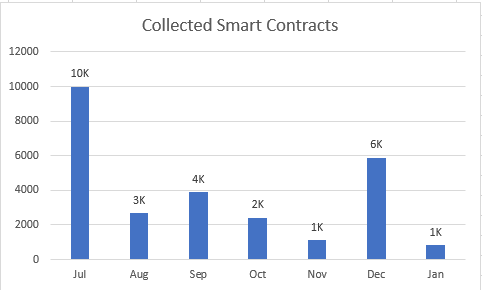
\includegraphics[width=\linewidth]{img/collected_contracts.PNG}
  \caption{An overview of the amount of contracts collected each month. The collection started in July which is the reason for the initial 10,000 contracts. Interesting to mention is that starting mid-september, Etherscan has reduced the available verified smart contracts to download to only 5000. The small collection of January is due to only retrieving the database once at the start of the month.}
  \Description{Smart Contracts per month}
  \label{fig:database}
\end{figure}
\subsection{Method}
Using the available API it is now possible to retrieve all source codes for each contract. To retrieve information from the Etherscan API an API key is needed which can be made on Etherscan, after that we can use following API endpoint  [\ref{lst:api}] for each contract address. 

\begin{lstlisting}[language=Solidity, caption=Api call, label={lst:api}]
https://api.etherscan.io/api
   ?module=contract
   &action=getsourcecode
   &address=0xaddress // The contract address
   &apikey=YourApiKeyToken // Your API key
\end{lstlisting}

Calling this will give a json response with following information from which
we collect all source codes, contract names and the compiler version. For a more indepth explanation of how the API works we refer to the documentation made available on Etherscan \cite{etherscan_api}. 
\begin{lstlisting}[language=json,firstnumber=1]
{
   "status":"1",
   "message":"OK",
   "result":[
      {
         "SourceCode": "Source code"
         "ABI":"[The ABI Interface]"
         "ContractName":"The Contract Name",
         "CompilerVersion":"The Compiler Version",
         "OptimizationUsed":"1",
         "Runs":"200",
         "ConstructorArguments":"Constructor arguments",
         "EVMVersion":"Default",
         "Library":"",
         "LicenseType":"",
         "Proxy":"0",
         "Implementation":"",
         "SwarmSource":""
      }
   ]
}
\end{lstlisting}

\section{Analysis and Results}

The aim of these experiments will be to have a preliminary analysis of the contracts and to detect potential reentrancy threats where the call function is present. We start with a total of 26,800 unique verified smart contracts. 



The first experiment is to take a look at the lines of code of these verified smart contracts and gather some statistics.

After an initial calculation we get the following values for the amount of lines of code, we notice their is a huge standard deviation in comparison with the median.
\begin{itemize}
    \item Average: 739
    \item Median: 547
    \item Standard deviation: 678
    \item Min LOC: 1
    \item Max LOC: 9452
\end{itemize}

Another piece of data we will take a look at are the different versions of Solidity used in each contract. We plot the 30 most used versions in the following bar chart Figure \ref{fig:compiler} and also plot these versions by only looking at the major version \ref{fig:compiler_major}. We can notice that three versions are used in more than half of the database namely v0.6.12, v0.8.4 and v0.8.7. The specific amount of contracts for each version and the percentage of the database that have that contract version can be found in Table \ref{tab:versions}
\begin{figure}[h]
  \centering
  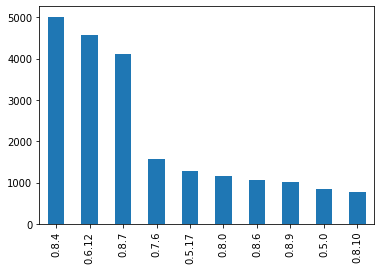
\includegraphics[width=\linewidth]{img/versions_v3.png}
  \caption{An overview of the top 10 solidity compiler versions used and the amount of contracts in the database that use that specific version. }
  \Description{Solidity Compiler Version}
  \label{fig:compiler}
\end{figure}

\begin{figure}[h]
  \centering
  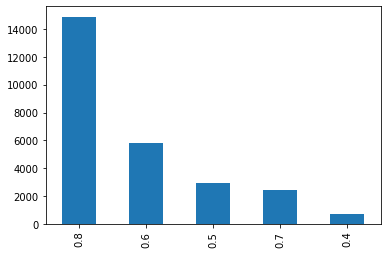
\includegraphics[width=\linewidth]{img/major_versions.png}
  \caption{An overview of the top solidity compiler versions used and the amount of contracts in the database that use that version, where we go into a higher level and only look at the major version. }
  \Description{Solidity Compiler Version}
  \label{fig:compiler_major}
\end{figure}

\begin{table}
  \caption{Compiler Versions}
  \label{tab:versions}
  \begin{tabular}{ccl}
    \toprule
    Solidity Version & \# Contracts & \% Percentage\\
    \midrule
    0.8.4&5015&18.71\%\\
    0.6.12&4587&17.12\%\\
    0.8.7&4103&15.3\%\\
    0.7.6&1564&5.84\%\\
    0.5.17&1278&4.77\%\\
    0.8.0&1166&4.35\%\\
    0.8.6&1060&3.96\%\\
    0.8.9&1008&3.76\%\\
    0.5.0&857&3.20\%\\
    0.8.10&768&2.87\%\\
    Other&5394&20.13\%\\
  \bottomrule
\end{tabular}
\end{table}

\begin{table}
  \caption{Compiler Versions (Major)}
  \label{tab:versions}
  \begin{tabular}{ccl}
    \toprule
    Solidity Version & \# Contracts & \% Percentage\\
    \midrule
    0.8&14869&55.48\%\\
    0.6&5839&21.79\%\\
    0.5&2954&11.02\%\\
    0.7&2454&9.16\%\\
    0.4&684&2.55\%\\
  \bottomrule
\end{tabular}
\end{table}
We will now dive deeper into the source contracts themselves and have a look at the different functionality, more specifically we will count the amount of times we find a call, send, and transfer function which as mentioned earlier are the main methods to exchange Ether in a Solidity smart contract. We will also calculate the amount of times a require, assert and throw function has been called in order to see how many of this contracts make use of guards. Table \ref{tab:stats} shows us the different statistics for the collected database. We notice that almost all contracts have some form of a guard pattern with a require function. Only 270 contracts actually have a call.value function which shows us that they may have a potential reentrancy attack. 

\begin{table}
  \caption{Statistics}
  \label{tab:stats}
  \begin{tabular}{ccl}
    \toprule
    Function & \# Contracts & \# Functions\\
    \midrule
    Call&270&384\\
    Send&9176&17,814\\
    Transfer&647&1059\\
    Require&26,191&622,701\\
    Assert&7279&10,507\\
    Throws&4174&10,590\\
    \toprule
    Function & Avg/contract\\
    \midrule
    Call&0.014\\
    Send&0.665\\
    Transfer&0.0396\\
    Require&23.235\\
    Assert&0.392\\
    Throws&0.395\\
  \bottomrule
\end{tabular}
\end{table}
The next experiment will focus more on those contracts that contain a call.value function, all previous statistics will be recalculated for only the smart contracts containing a call.value function to see if there are any similarities but first we will take a look at which version is used most in these contracts.
Figure \ref{fig:call_version}. The most used version is v0.5.17 which was the 5th most used version in all our contracts. A more interesting finding is that there are only 4 contracts above v0.6 that contain a call function of which 3 are from the compiler version that was most used by the complete database namely v0.8.4. For the line of code statistics we get the following values:
\begin{itemize}
    \item Average: 1050
    \item Median: 761
    \item Standard deviation: 1079
    \item Min: 31
    \item Max: 6535
\end{itemize}
We notice that these smart contracts on average are of a relatively bigger size in comparison with a regular contract.
Table \ref{tab:call} will now show us different statistics for this specific selection of contracts that only contain a call.value function. In this sub selection of contracts a call function is called about 1.4 times on average in a contract and a total of 384 call functions were called in 270 contracts with the highest amount of calls in a single contract being 14. An interesting thing to note is that the average amount of guards is higher for these contracts, this shows us that a guard pattern has been potentially used in cases where a call.value function has been used and are signs that most of these contracts are probably correctly implemented. 

\begin{figure}[h]
  \centering
  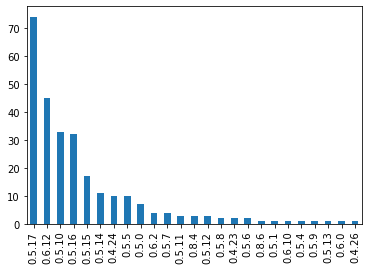
\includegraphics[width=\linewidth]{img/versions_call_v3_total.png}
  \caption{An overview of all the specific compiler versions used in contracts that contain a call.value function. }
  \Description{Solidity Compiler Version}
  \label{fig:call_version}
\end{figure}

\begin{table}
  \caption{Statistics of Contracts containing call function}
  \label{tab:call}
  \begin{tabular}{ccl}
    \toprule
    Function & \# Contracts & \# Functions\\
    \midrule
    Send&153&495\\
    Transfer&18&51\\
    Require&270&11932\\
    Assert&192&333\\
    Throws&163&324\\
    \toprule
    Function & Avg/contract\\
    \midrule
    Send&1.83\\
    Transfer&0.19\\
    Require&44.19\\
    Assert&1.23\\
    Throws&1.2\\
  \bottomrule
\end{tabular}
\end{table}

We will do a similar analysis on both the send and transfer function. Looking at the versions in Figure \ref{fig:send_version} we can see that for the send function the top 5 versions are completely similar to the top 5 versions of the whole contract database. This is partly due to the fact that 66\% of the contracts of our whole database have a send function. If we look at the versions of transfer in Figure \ref{fig:transfer_version} we notice that both v0.8.4 and 0.6.12 are not even in the top 10 versions which is interesting. A version that also showed up in the top 10 of call versions namely v0.4.24 shows up here. This signifies that both call and transfer functions were used more often in v0.4 and that since then there was a shift to the send function. 

\begin{figure}[h]
  \centering
  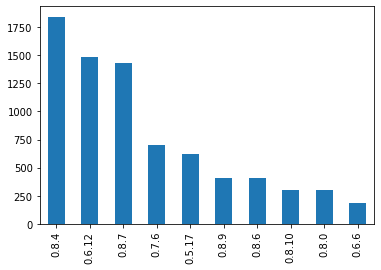
\includegraphics[width=\linewidth]{img/sends_versions.png}
  \caption{An overview of all the specific compiler versions used in contracts that contain a send function. }
  \Description{Solidity Compiler Version (Sends)}
  \label{fig:send_version}
\end{figure}

\begin{figure}[h]
  \centering
  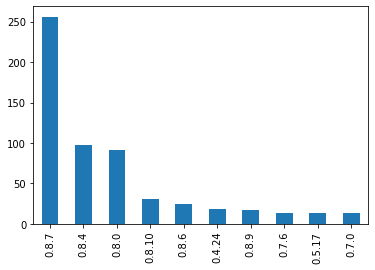
\includegraphics[width=\linewidth]{img/transfers_versions.png}
  \caption{An overview of all the specific compiler versions used in contracts that contain a transfer function. }
  \Description{Solidity Compiler Version (Transfers)}
  \label{fig:transfer_version}
\end{figure}

If we calculate the LOC statistics for both contracts containing send functions and contracts containing transfer functions we get the statistics in Table \ref{tab:loc}. Contracts containing a transfer function seem to be a lot longer on average (almost twice as long) in comparison with the average length of a smart contract. A contract containing a send function is pretty similar in length in comparison with the average smart contract.
\begin{table}
  \caption{LOC Statistics for send and transfer}
  \label{tab:loc}
  \begin{tabular}{ccl}
    \toprule
    Statistic & Send & Transfer\\
    \midrule
    Average&832&1453\\
    Mean&553&1378\\
    Std Dev&741.78&841.18\\
    Min&10&20\\
    Max&9452&9452\\
  \bottomrule
\end{tabular}
\end{table}

Of all contracts containing a send functions there are almost on average two send functions per contract with the highest amount of send functions used in any contract being 68. This is by far the most used way of transferring Ether in the database that we collected. The transfer function is present in a lot less contracts but when it is used, the average of times it is in a contract is around 1.63 times with the highest amount being 12. 
We will now look at the different functions present in both cases in a similar way we did for the call function for which the results can be found in Table \ref{tab:send} and Table \ref{tab:transfer}. For the contracts containing a send function we notice that they almost always include atleast one require guard as well. The average of require guards used in a contract containing a transfer function is however higher in comparison with the average of contracts that contain a send function. We can also see that the average of both assert guards and throws are higher for contracts containing a send function than the transfer function. If we now compare some of these statistics to the numbers of the contracts containing a call function we immediately see that those contracts have a lot more guards. These due to the fact that both transfer and send are considered safer functions and thus a call function by design will need to utilize more guards for it to not be exploited.

\begin{table}
  \caption{Statistics of Contracts containing send function}
  \label{tab:send}
  \begin{tabular}{ccl}
    \toprule
    Function & \# Contracts & \# Functions\\
    \midrule
    Call&153&226\\
    Transfer&107&251\\
    Require&9060&256835\\
    Assert&2722&4789\\
    Throws&1507&4338\\
    \toprule
    Function & Avg/contract\\
    \midrule
    Call&0.0246\\
    Transfer&0.0274\\
    Require&27.9898\\
    Assert&0.5219\\
    Throws&0.4727\\
  \bottomrule
\end{tabular}
\end{table}

\begin{table}
  \caption{Statistics of Contracts containing transfer function}
  \label{tab:transfer}
  \begin{tabular}{ccl}
    \toprule
    Function & \# Contracts & \# Functions\\
    \midrule
    Call&18&20\\
    Send&107&234\\
    Require&647&25058\\
    Assert&63&166\\
    Throws&53&224\\
    \toprule
    Function & Avg/contract\\
    \midrule
    Call&0.0309\\
    Send&0.3616\\
    Require&38.7295\\
    Assert&0.2566\\
    Throws&0.3462\\
  \bottomrule
\end{tabular}
\end{table}
\section{Related work}


Juels, Kosba and Shi\cite{criminal} investigate the risk of smart contracts fueling new criminal ecosystems . They show how a Criminal Smart Contract can facilitate leakage of confidential information, theft of cryptographic keys and more, showing the urgency of creating safeguards against these CSCs. They look at questions like how practical these new crimes will be, whether these CSCs enable a wider range of new crimes in comparison to earlier cryptocurrencies such as Bitcoin and what advantages they offer to criminals in comparison with the conventional online systems. 


Luu et al.  \cite{smarter} also investigate and introduce several security problems to manipulate smart contracts in an attempt to gain profit and propose ways to enhance the operational semantics of Ethereum. A focus is put on the semantic gap between the assumption contract writers make about the underlying execution semantics and the actual semantics of the contract are made as a reason for these security flaws. A tool OYENTE is also provided to detect bugs which is a symbolic execution tool. The model works directly with Ethereum virtual machine byte code and thus does not have a need for a higher level representation such as Solidity. An evaluation of OYENTE on 19366 smart contracts is given where 8333 contracts were documented as potentially having bugs.

Mense and Flatscher \cite{security} summarize known vulnerabilities found by literature research and analysis such as external calls, gasless sends, mishandled exceptions and reentrancy. They also compare code analysis tools for their ability to identify vulnerabilities in smart contracts based on a taxonomy for vulnerabilities. The results of their paper show that reentrancy ranks the highest among the vulnerabilities that they have discussed and is detected by most of the tools used. They then delve deeper into the DAO hack aswell. 


Liu et al. \cite{reguard} present ReGuard which is a fuzzing-based analyzer to automatically detect reentrancy bugs in Ethereum smart contracts. They iteratively generate random (but diverse) transactions, this is called fuzz testing. Then based on the runtime they will identify reentrancy vulnerabilities in a contract. How the architecture works is they parse a smart contracts source or binary code to an intermediate representation which will then be transformed to C++, keeping the original behavior. Together with a runtime library, ReGuard executes the contract and runs an analysis of the operations for any reentrancy attacks.


SmartCheck is an extensible static analysis tool to detect code issues in Solidity by Tikhomirov et al.\cite{smartcheck} where they translate Solidity into an XML-based representation and check it against XPath patterns. They also used a real world dataset to evaluate their tool and also make a comparison to the earlier mentioned Oyente. 


Samreen and Alalfi  \cite{survey} explain eight vulnerabilities by looking at past exploitation case scenarios and review some of the available tools and applications to detect these vulnerabilities. For each case they discuss the vulnerability exploited, the tactic used as well as the financial loss what happened. A coverage is given of some preventive techniques as protection against some of these exploits. The tools/frameworks they discuss adopt either a form of static analysis such as symbolic execution and control flow graph construction or dynamic analysis such as the fuzzing testing or tracing the sequence of instructions that are executed at run time. 

Tantikul and Ngamsuriyaroj \cite{icissp20} investigate a more recent state of the vulnerabilities of smart contracts. Their research consists of going through a database of verified smart contracts and checking common occurrences as well as trends of vulnerabilities. An analysis is done using both Oyente and Smartcheck and common characteristics of vulnerable smart contracts are identified. A correlation computation is done via Pearson's correlation in order to detect how often any pair of vulnerabilities will be found on the same smart contract. Their results show that overflow and underflow have the highest correlation. Another relation found is the timestamp dependency and transaction ordering which might be caused by malicious miners.  

Bragagnolo, Rocha, Denker and Ducasse \cite{rocha} address the lack of inspectability of a deployed smart contact. They do this by analyzing the state of the contract using different decompilation techniques. Their solution SmartInspect is an inspector based on pluggable property reflection. Their approach of utilizing mirrors generated from an analysis of Solidity source code allows access to unstructured information from a deployed smart contract in a structured way. This can be done without a need to redeploy or develop additional code for decoding. 

Wang et al. \cite{contractward} evaluate a set of real-world smart contracts with ContractWard which uses machine learning techniques to detect vulnerabilities in smart contracts. Their idea was proposed due to existing detection methods being mainly based on symbolic execution or analysis which are very time-consuming. The system extracts dimensional bigram features from simplified operation codes to construct a feature space and is able to get a predictive recall and precision of over 96\% based on their dataset of 49502 smart contracts on 6 vulnerabilities.

A deep-learning based approach is used by Qian et al. \cite{automated}. The aim is to precisely detect reentrancy bugs using a bidirectional long-short term memory with attention mechanism. They also propose using a contract snippet as another way to represent a smart contract only capturing key semantic sentences which contain related and critical information such as control flow and data dependencies. These are then used as input to the sequential models. They show that this deep-learning approach outperforms other state-of-the-art smart contract vulnerability tools.

Slither by Feist et al. \cite{slither} is a static analysis framework that converts Solidity smart contracts into an intermediate representation which they call SlithIR. Static Single Assignment forms are used aswell as a reduced instruction set for ease of implementation. Their framework has use cases in automated detection of vulnerabilities, detection of code optimization opportunities, improvement of clarity and ease of understanding of the contracts. An evaluation of the proposed frameworks capabilities is done using a set of real-world smart contracts. 

%%
%% The next two lines define the bibliography style to be used, and
%% the bibliography file.


\bibliographystyle{ACM-Reference-Format}
\bibliography{references}
\end{document}
\endinput
%%
%% End of file `sample-xelatex.tex'.
